\documentclass{article}
\usepackage[backend=biber]{biblatex}
\usepackage[]{hyperref}
\usepackage{graphicx}
\usepackage{booktabs}
\usepackage{siunitx}
\usepackage[]{amsmath}
\addbibresource{bibliography.bib}
\author{De Trane Giorgio\\s275514}
\title{\textbf{Esercitazioni Strutture\\per Veicoli Spaziali}}

\begin{document}
    \maketitle
    \begin{center}
        \includegraphics[width=0.8\textwidth]{polito_logo.png}
        \linebreak
        \linebreak
        \textit{Anno accademico\\2020-2021}
    \end{center}
    \pagebreak
    \section{Esercitazione 1}
    L'esercitazione é svolta utilizzando uno script in Fortran, messo a disposizione
    in un archivio denominato \textit{MUL2} \autocite*{MUL2} e contenente anche un file di input ad hoc, in formato \textit{.dat},
    oltre a degli utili script di esempio per \textit{gnuplot} \autocite*{gnuplot}, un libre software utilizzato poi per plottare tutti i grafici che seguono.
    \\
    \linebreak 
    Sono state fatte diverse assunzioni per tutta 
    l'esercitazione:
    \begin{itemize}
        \item La depressurizzazione é \textit{lenta} 
        ($\displaystyle t > 10\, s$ \ )
        \item Il volume delle camere é \textit{costante}
        \item Il volume dell'atmosfera é supposto \textit{infinito}
        \item L'aria é trattata come \textit{gas ideale}
        \item Si utilizza un modello 0D, ossia con
              proprietá uniformi per tutta l'aria contenuta nel volume in analisi
        \item La quota rimane \textit{costante} durante la depressurizzazione
        \item L'effetto dell'umiditá relativa e dei calori latenti vengono trascurati
        \item Il modello utilizzato é di tipo quasi-stazionario, implementato attraverso un 
              \textit{algoritmo numerico}

    \end{itemize}

    \begin{center}
        \includegraphics[width=0.75\textwidth]{MUL2_feedback.png}\\
        \textit{Fig1: stdout dello script}
    \end{center}
    




    \pagebreak

        \subsection{Esempio}
        Il caso esaminato é quello dell'Esempio 2, i cui dati sono quelli
        forniti di default nel file input.dat .\\
        La configurazione in esame consiste in due camere comunicanti attraverso
        una ventilazione passiva, con un breach sull'ambiente esterno. 
        \begin{center}
            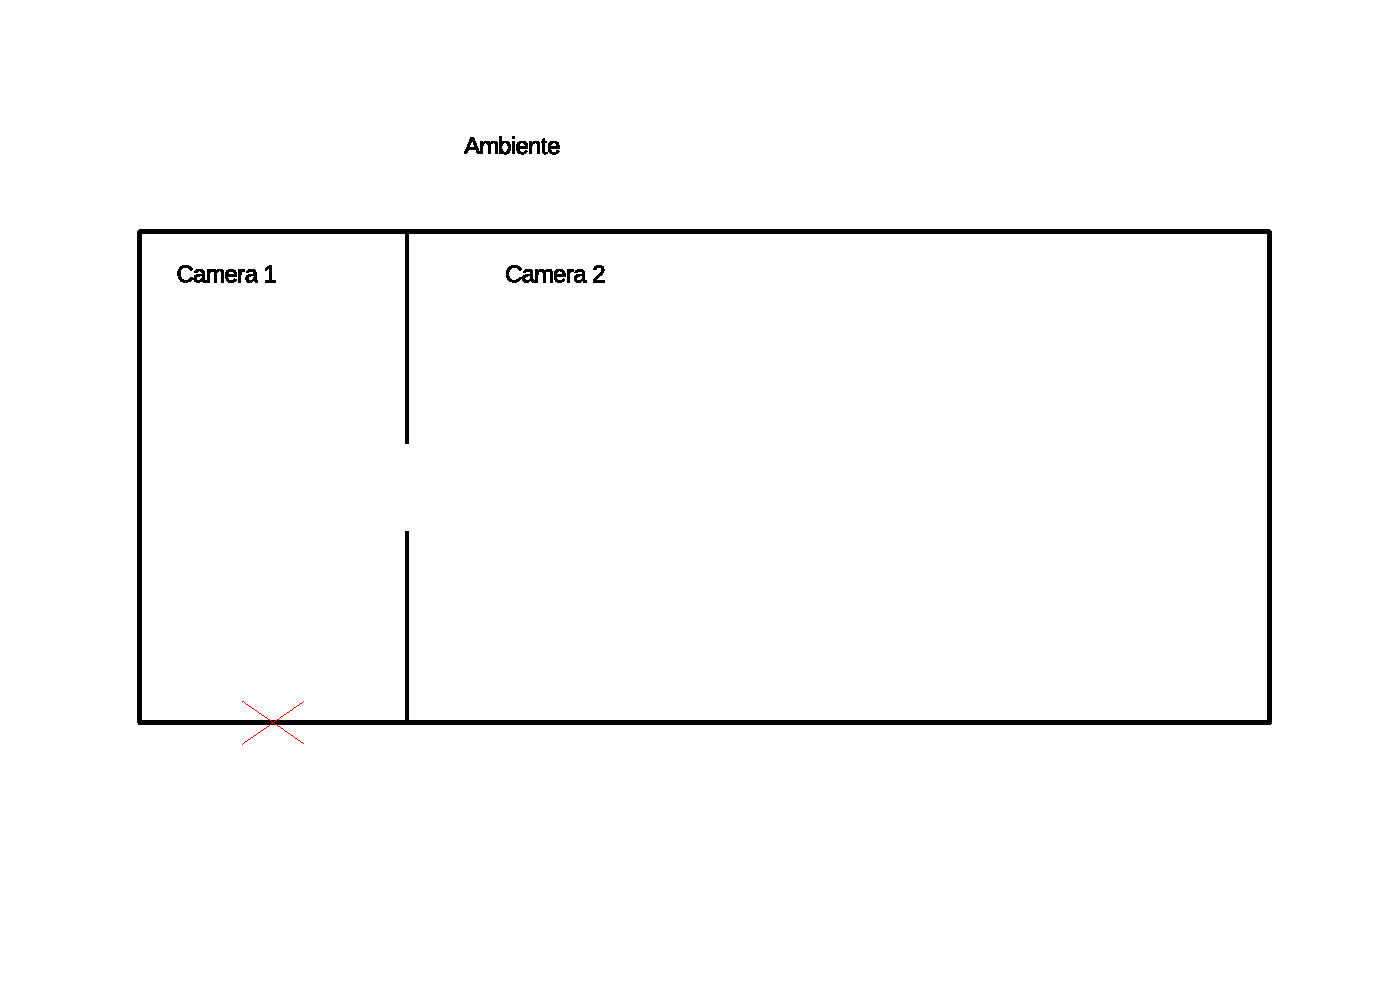
\includegraphics[width=0.7\textwidth]{ES1_Esempio2.eps}\linebreak
            \textit{Fig2: Esempio2}
        \end{center}

        \textbf{\textit{DATI}}
        \begin{itemize}
            \item $\displaystyle T_0 = -10\,C;$ \
            \item $\displaystyle T_{c0} = 23\,C;$ \
            \item $\displaystyle p_0 = 62.8812\,kPa;$ \
            \item $\displaystyle p_{c0} = 117.0162\,kPa;$ \
            \item $\displaystyle V_{c1} = 4\,m^3;$ \
            \item $\displaystyle V_{C2} = 16\,m^3;$ \
            \item $\displaystyle A_{1-0} = 0.2\,m^2;$ \
            \item $\displaystyle A_{1-2} = 0.5\,m^2;$ \
            \item $\displaystyle CD_{1-0} = 0.8;$ \
            \item $\displaystyle CD_{1-2} = 0.7;$ \
        \end{itemize}
        \pagebreak

        \textbf{RISULTATI}
        \\ \\
        Sono riportati i grafici ottenuti plottando i file di output
        generati dallo script.
        \begin{center}
            \includegraphics[width=0.65\textwidth, angle=-90]{MUL2/p.eps}\\
            \textit{Fig.3: Pressioni di entrambe le camere nel tempo}
            \includegraphics[width=0.65\textwidth, angle=-90]{MUL2/Dp.eps}\\
            \textit{Fig4: Gradiente di pressione tra le due camere}
        \end{center}

        \pagebreak
        \printbibliography
\end{document}